\documentclass[11pt]{article}

\title{% 
Tenzor link analysis}
\author{Bruno Fabuli\'{c}, Helena Marciu\v{s}, Dora Parma\'{c}}

\usepackage{amsmath}
\usepackage{amsthm}
\usepackage{amssymb}
\usepackage{esvect}
\usepackage[utf8]{inputenc}
\usepackage{amsfonts}
\usepackage{hyperref}
\usepackage{listings}
\newcommand\eref[1]{(\ref{#1})}
\usepackage{enumitem}
\usepackage[croatian]{babel}
\usepackage{graphicx}
\graphicspath{ {./images/} }
\hypersetup{
    urlcolor=black
}
\hypersetup{%
    pdfborder = {0 0 0}
}
\newtheorem{theorem}{Teorem}[section]
\newtheorem{prop}{Propozicija} [section]
\newtheorem{corollary}{Korolar}[theorem]
\usepackage{listings}
\usepackage{biblatex}
\addbibresource{dokumentacija.bib}
\newcommand{\norm}[1]{\left\lVert#1\right\rVert}
\usepackage{algorithm}
\usepackage[noend]{algpseudocode}
\algdef{SE}[DOWHILE]{Do}{doWhile}{\algorithmicdo}[1]{\algorithmicwhile\ #1}%


\begin{document}
	\maketitle
	\pagenumbering{gobble}
	\newpage
	\hypersetup{linkcolor=black}
	\tableofcontents
	\pagenumbering{roman}
\newpage
\hypersetup{linkcolor=blue}
\pagenumbering{arabic}


\section{Uvod}
Kako se veličina Weba povećava, postaje sve važnije analizirati strukturu linkova uzimajući u obzir i kontekst.
Multilinearna algebra pruža novi alat za obuhvaćanje teksta poveznice i drugim informacija koji se koriste u drugih metodama analize poveznica kao što je HITS algoritam.

Algoritam kojeg proučavamo naziva se Topical HITS ili TOPHITS. On je generalizacija Kleinbergovog HITS modela. TOPHITS dodaje 3. dimenziju za oblikovanje tenzora susjedstva koji uključuje i tekst poveznice. Ova dodatna informacija pruža način za obuhvaćanje konteksta uz izračunavanje autoriteta i hubova, što je postignuto 3D Parallel Factors (PARAFAC) dekompozicijom, više-dimenzionalni analogon SVD dekompozicije.
Dodavanje 3. dimenzije znatno poboljšava primjenjivost HITS-a, zato što se TOPHITS analiza može izvoditi unaprijed i offline. Također, TOPHITS otkriva latentno grupiranje stranice i informacija.

U ovom seminaru, opisat ćemo brži matematički algoritam za izračunavanje TOPHITS algoritma na podatcima.

\begin{figure}[hbt!]
    \centering
    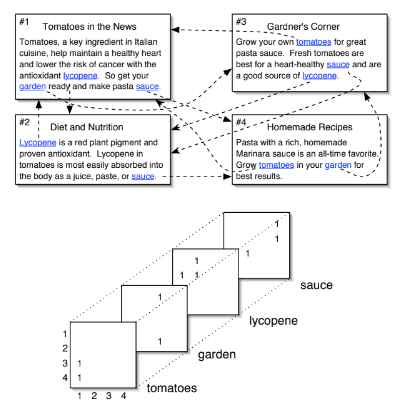
\includegraphics[width= \textwidth, height=85mm]{slika1.png}  
    \caption{TOPHITS analizira 3D tenzor koji reprezentira kolekciju web stranica}
\end{figure}

\newpage
\section{Usporedba HITS i TOPHITS algoritma}
Mnoge metode za analizu weba, poput PageRanka i HITS-a bazirane su na matrici susjedstva grafa kolekcije web stranica. PageRank rezultati dani su ulazima glavnog svojstvenog vektora Markovljeve matrice vjerojatnosti. S druge strane, HITS računa hubove i autoritete za svaki vrh i oni odgovaraju glavnom lijevom i desnom singularnom vektoru matrice susjedstva.
Zanimljivo svojstvo HITS-a, što ne dijeli s PageRankom jest da se višestruki parovi singularnih vektora mogu razmatrati.

\subsection{HITS}
\begin{flushleft}
Neka je $I$ broj stranica u našem podgrafu. Svaka stranica ima hub-score $h$ i autoritet-score $a$ koje računamo iterativno na sljedeći način:
\end{flushleft}
\begin{equation}\label{eq:1}
    \boldsymbol{h}_{i}^{(t+1)} = \displaystyle\sum_{i \rightarrow j} \boldsymbol{a}_j^{t}
\end{equation}

\begin{equation}\label{eq:2}
    \boldsymbol{a}_{j}^{(t+1)} = \displaystyle\sum_{i \rightarrow j} \boldsymbol{h}_i^{t+1}
\end{equation}

\begin{flushleft}
Nakon svake iteracije, normaliziramo $h$ i $a$. To znači da je hub-score stranice i jednak sumi autoritet-scorova svih stranica na koje pokazuje. Slično, autoritet-score stranice i jednak je sumi hub-scorova svih stranica koje pokazuju na nju.
\end{flushleft}

\begin{flushleft}
Zapišimo to matrično. Neka je $I \times I$ matrica susjedstva $\boldsymbol{X}$ definirana  kao:
\end{flushleft}
\begin{equation}
    X_{i,j} =  \left\{
	\begin{array}{ll}
		1  & \mbox{ako stranica i pokazuje na stranicu j} \\
		0 & \mbox{inače }
	\end{array}
\right.
\end{equation}
\begin{flushleft}
Tada jednadžbe \ref{eq:1} i \ref{eq:2} postaju:
\end{flushleft}
\begin{equation}
    \boldsymbol{h}^{(t+1)} = \boldsymbol{X} \boldsymbol{a}^{(t)} \\ , \\
    \boldsymbol{a}^{(t+1)} = \boldsymbol{X}^{T} \boldsymbol{h}^{(t+1)}
\end{equation}

\begin{flushleft}
Prvih R faktora singularne dekompozicije of $\boldsymbol{X}$ proizvodi najbolju R-rang aproksimaciju, odnosno možemo aproksimirati $\boldsymbol{X}$ kao:
\end{flushleft}
\begin{equation}
    \boldsymbol{X \approx H \Sigma A^{T} \equiv \sum_{r = 1}^{R} \sigma_{r} h_{r} \circ a_{r}}
\end{equation}

\begin{raggedleft}
Vrijedi $\Sigma = diag\{\sigma_{1} \ldots \sigma_{R}\}$ i za singularne vrijednosti pretpostavljamo $\sigma_{1} \ge \sigma_{2} \ge \ldots \ge \sigma_{R} > 0 $ i gdje su $\boldsymbol{h_r}$ i $\boldsymbol{a_r}$ odgovarajući singularni vektori. Matrice $\boldsymbol{H} i  \boldsymbol{A}$ su veličine $I \times R$ i imaju ortonormalna polja. To možemo zamisliti kao aproksimaciju matrice $\boldsymbol{X}$ sumom $R$ 1 ranga vanjskog produkta, kako je prikazano na  (\ref{figure:2}) Glavni par singularnih vektora $\boldsymbol{h_1}$ i $\boldsymbol{a_1}$ pruža hub i aurotitet rezultate za dominantnu temu u kolekciji web stranica. Drugim riječima, stranice koje imaju najveće rezultate $\boldsymbol{h_1}$ su najbolji hubovi za dominantnu temu, a stranice koje imaju najveće rezultate u $\boldsymbol{a_1}$ su najbolji autoriteti. 
\end{raggedleft}

\begin{figure}[hbt!]
    \centering
    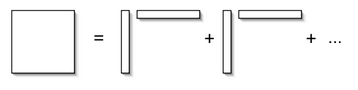
\includegraphics[width= \textwidth]{svd.png}  
    \caption{SVD dekompozicija}
    \label{figure:2}
\end{figure}

\newpage
\subsection{TOPHITS}
\begin{flushleft}
Ilustrirajmo sada TOPHITS algoritam. On proizvede trojke 
$\boldsymbol{h_1}$,  $\boldsymbol{a_1}$, $\boldsymbol{t_1}$  gdje $\boldsymbol{u}$ i $\boldsymbol{v}$ predstavljaju hub i aurotitet rezultate, a $\boldsymbol{t}$  term rezultate.
\end{flushleft}

\begin{flushleft}
Slično kao HITS, rezultati se mogu dobiti iterativno. Neka je $I$ broj stranica, a $K$ broj termova. Tada je:
\end{flushleft}

\begin{equation}\label{eq:3}
    \boldsymbol{h}_{i}^{(t+1)} = \displaystyle\sum_{i \xrightarrow{\text{k}} j} \boldsymbol{a}_j^{t} \boldsymbol{t}_{k}^{(t)} \hspace{1cm} \text{za} \hspace{0.3cm} i = 1, \ldots, I
\end{equation}

\begin{equation}\label{eq:4}
    \boldsymbol{a}_{j}^{(t+1)} = \displaystyle\sum_{i \xrightarrow{\text{k}} j} \boldsymbol{h}_i^{t+1} \boldsymbol{t}_{k}^{(t)} \hspace{1cm} \text{za} \hspace{0.3cm} j = 1, \ldots, I
\end{equation}

\begin{equation}\label{eq:5}
    \boldsymbol{t}_{k}^{(t+1)} = \displaystyle\sum_{i \xrightarrow{\text{k}} j} \boldsymbol{a}_j^{t+1} \boldsymbol{h}_i^{t+1} \hspace{1cm} \text{za} \hspace{0.3cm} k = 1, \ldots, I
\end{equation}

\begin{raggedleft}
Kao i kod HITS-a, normaliziramo vrijednosti nakon svake iteracije.
\end{raggedleft}

\begin{flushleft}
Zapišimo to u tenzor formi. Neka je $\boldsymbol{X}$ $I \times I \times K $ tenzor susjedstva podgrafa definiran kao:
\end{flushleft}

\begin{equation}\label{eq:6}
    X_{i,j, k} =  \left\{
	\begin{array}{ll}
		1  & \mbox{ako stranica i pokazuje na stranicu j koristeći term k} \\
		0 & \mbox{inače }
	\end{array}
\right.
\end{equation}

\begin{flushleft}
Tada se jednadžbe \ref{eq:3}, \ref{eq:4} i \ref{eq:5} mogu zapisati kao:
\end{flushleft}
\begin{equation}
    \boldsymbol{h}^{(t+1)} = \boldsymbol{X} \overset{-}{\times}_{2} \boldsymbol{a}^{(t)}  \overset{-}{\times}_{3} \boldsymbol{t}^{(t)}
\end{equation}
\begin{equation}
    \boldsymbol{a}^{(t+1)} = \boldsymbol{X}^{T}\overset{-}{\times} \boldsymbol{h}^{(t+1)} \overset{-}{\times}_{3} \boldsymbol{t}^{(t)}
\end{equation}
\begin{equation}
    \boldsymbol{t}^{(t+1)} = \boldsymbol{X}^{T}\overset{-}{\times}_{1} \boldsymbol{h}^{(t+1)} \overset{-}{\times}_{2} \boldsymbol{a}^{(t)}
\end{equation}

\begin{flushleft}
Ovdje notacija $\boldsymbol{X}\overset{-}{\times}_{i} \boldsymbol{x}$ znači množenje  tenzora $\boldsymbol{X}$ vektorom $x$ u dimenziji i.
\end{flushleft}
\begin{flushleft}
Tada se aproksimacija tenzora $\boldsymbol{X}$ PARAFAC dekompozicijom može dobiti kao:
\end{flushleft}
\begin{equation}
    \boldsymbol{\mathcal{X} \approx \lambda [\![ H, A, T ]\!] \equiv \sum_{r = 1}^{R} \lambda_{r} h_{r} \circ a_{r} \circ t_{r}}
\end{equation}

\begin{raggedleft}
Ovdje pretpostavljamo $\lambda_{1} \ge \lambda_{2} \ge \ldots \ge \lambda_{R}$.
Matrice $\boldsymbol{H, A, T}$ imaju polja duljine 1, ali suprotno od SVD-a, nisu generalno ortonormalne. PARAFAC dekompozicija aproksimira tenzor $\boldsymbol{\mathcal{X}}$ sumom , kao što je  prikazano na (\ref{fig:3}) .
\end{raggedleft}

\begin{figure}[hbt!]
    \centering
    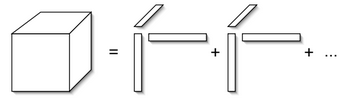
\includegraphics[width= \textwidth]{parafac.png}  
    \caption{PARAFAC dekompozicija}
    \label{fig:3}
\end{figure}

\begin{flushleft}
Glavna trojka PARAFAC vektora $\boldsymbol{h_1}$,  $\boldsymbol{a_1}$, $\boldsymbol{t_1}$  pruža hub i aurotitet rezultate za dominantnu temu u kolekciji web stranica (na isti način kao što je prethodno opisano kod HITS-a), te term rezultate. Drugim riječima, termi koji imaju najveće rezultate $\boldsymbol{t_1}$ su najdeskriptivniji termi.
\end{flushleft}
\begin{flushleft}
Suprotno SVD-u, nema garancije da će PARAFAC aproksimacija biti optimalna, te vektori nisu ortogonalni.
\end{flushleft}

\newpage
\subsubsection{TOPHITS ukratko}
Ideja iza TOPHITSa je sljedeća: pretpostavimo da analiziramo kolekciju $I$ web stranica imajući ukupno $K$ termova u tekstu poveznica svih poveznica. Tada je $I \times I \times K$ tenzor susjedstva $\boldsymbol{\mathcal{X}}$ definiran kao u (\ref{eq:3}). Primijetimo da je tenzor $\boldsymbol{\mathcal{X}}$ rijedak zato što većina stranica pokazuje samo na na nekoliko drugih stranica u kolekciji, a svaki  link koristi samo nekoliko termova. Stoga je realno za očekivati da je broj ne-nul elemenata u $\boldsymbol{\mathcal{X}}$ jednak $O(I)$.
\newline
\vskip
Uzimajući u obzir $R > 0$ (broj različitih grupiranja podataka), TOPHITS algoritam pronađe matrice $\boldsymbol{H} \textbf{i} \boldsymbol{A}$, veličina $I \times R$, i matricu $\boldsymbol{T}$ veličine $K \times R$.
Svaka trojka $\{ \boldsymbol{h_r}, \boldsymbol{a_r}, \boldsymbol{t_r}\}$, za $r = 1 \ldots R$ definira grupiranje hubova, autoriteta i terma uzimajući u obzir ulaze s najvećom vrijednosti u svakom vektoru; vrijednost $\lambda_{r}$ definira težinu grupiranja. (Bez smanjenja općenitosti, pretpostavljamo da su stupci naših matrica normalizirani.)
\newline
\vskip
TOPHITS je zapravo ekstenzija Kleinbergovog HITS algortma koja je koristila singularni vektor matrice hiperlinkova (2D tenzor) da bi proizvela skup hubova i autoriteta. Dodatak topic-vektora znači da je određivanje skupa singularnih vektora koji sadrže odgovor na upit zapravo promatranje koji topic-vektori imaju najveći score uključujući njihove autoritete i hubove.
Slično kao PageRank, TOPHITS je neovisan o upitima zato što se računanje značajnih vektora može obaviti unaprijed i offline.

\newpage
\section{Metodologija}
\subsection{PARAFAC model}
3D dekompozicija simultano je predložena sa strane Harshmana, koristeći ime "Parallel Factors ili PARAFAC" te sa strane Carroll i Chang, koristeći ime "Canonical Decomposition ili CANDECOMP".
Cilj je prikazati vektor reda $N$ kao sumu vektora vanjskog produkta kao što je prikazano na slici $\ref{fig:3}$.

Matematički, problem je zadan na sljedeći način.
Pretpostavimo da imamo tenzor $\boldsymbol{\mathcal{X}}$ veličine $I_{1} \times I_{2} \times \ldots \times I_{n}$ i željeni rang aproksimacije $R$. Tada želimo naći matrice $\boldsymbol{U} ^{n}$ veličine $I_{n} \times R$, za svaki $N = 1, \ldots, N$ i težinski vektor $\boldsymbol{\lambda}$ duljine $R$ tako da vrijedi:

\begin{equation}
    \boldsymbol{\mathcal{X} \approx \lambda [\![ U^{(1)}, U^{(2)}, \ldots, U^{(N)} ]\!] }
\end{equation}

Kruskalov operator $[\![.]\!]$ je skraćeni zapis sume ranga svih vanjskih produkata stupaca. Drugim riječima, 

\begin{equation}
    \mathrm{\lambda}[[\mathrm{U}^{(1)}, \mathrm{U}^{(2)}, \dots , \mathrm{U}^{(N)}]] \equiv \displaystyle\sum_{r=1}^{R} \lambda_{r} \mathrm{u}_{r}^{(1)} \circ \mathrm{u}_{r}^{(2)} \circ \dots \circ \mathrm{u}_{r}^{(N)}
\end{equation}

Bez smanjenja općenitosti, prepostavljamo da je $ \norm{\boldsymbol{u}_{r}^{(n)}} = 1$ za sve $r = 1, \ldots, R $ i $ n = 1, \ldots, N$. Povrh toga, preuredimo završno rješenje tako da vrijedi $\lambda_{1} \geq \lambda_{2} \geq \ldots \lambda_{R}$.

Cilj nam je riješiti problem minimizacije:

\begin{equation}
    \min \left\| \mathrm{X} - \mathrm{\lambda}[[\mathrm{U}^{(1)}, \mathrm{U}^{(2)}, \dots , \mathrm{U}^{(N)}]] \right\|^{2}
\end{equation}
s obzirom na $\mathrm{\lambda} \in \mathbb{R}^{R},~\mathrm{U}^{(n)} \in \mathbb{R}^{I_{n}\times R},~ n = 1,\dots , N$.

U slučaju TOPHITSA, $\boldsymbol{\lambda}$ je tenzor reda 3, tj $N = 3$ i vrijedi:
\begin{equation}
    \boldsymbol{H \equiv U^{(1)}}, 
    \boldsymbol{A \equiv U^{(2)}}, 
    \boldsymbol{T \equiv U^{(3)}}
\end{equation}

\subsection{Pohlepni PARAFAC}

Notacija $\boldsymbol{X}_{(n)}$ reprezentira n-to unfolding tenzora $\boldsymbol{\mathcal{X}}$. Drugim riječima, $\boldsymbol{X}_{(n)}$ predstavlja reorganizirane ulaze $\boldsymbol{\mathcal{X}}$ u matricu veličine $I_n \times J$, gdje je $J = \prod_{k=1, k \neq n} ^{N} I_{k}$ tako da su "vlakna" u dimenziji n uređena kao stupci matrice. Matematički imamo:

\begin{multline}
    [\boldsymbol{X}_{(n)}]_{i,j} = x_{i_1, i_2, \ldots, i_N} \\
    i = i_n, j = 1 + \sum_{k=1, k \neq n} ^{N} (i_n - 1) \prod{l=1, l\neq n} ^{k-1} I_l \\
    i \leq i \leq I_n, 1 \leq j \leq J
\end{multline}

\subsubsection{Pohlepni PARAFAC - pseudokod}

\begin{figure}[hbt!]
    \centering
    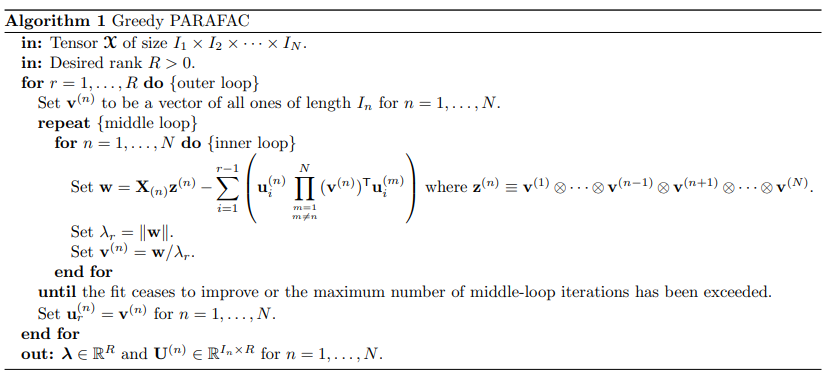
\includegraphics[width=420pt]{1.alg.png}  
    \label{fig:5}
\end{figure}

\newpage

\begin{enumerate}
    \item Vanjska petlja (po $r$) računa $\lbrace \mathrm{u}_{r}^{(1)}, \dots , \mathrm{u}_{r}^{(N)} \rbrace$\\
            Za svaki $r, r = 1, \dots ,N$, unutarnja petlja metodom alternirajućih najmanjih kvadrata minimizira 
     \item
        \begin{equation}
            \left\| \left(\bm{\mathrm X} - \displaystyle\sum_{i=1}^{r-1}\lambda_{i} \mathrm{u}_{i}^{(1)} \circ \dots \circ \mathrm{u}_{i}^{(N)}\right) - \left(\mathrm{v}^{(1)} \circ \dots \circ \mathrm{v}^{(N)}\right) \right\|
        \end{equation}
        po vektorima $\mathrm{v}^{(1)}, \dots , \mathrm{v}^{(N)}$\\
        Tada je 
            $\mathrm{u}_{r}^{(n)} = \mathrm{v}^{(n)},~ n = 1, \dots , N$

\end{enumerate}

\subsection{Alternirajući najmanji kvadrati za PARAFAC}

Češći pristup rješavanja PARAFAC dekompozicija je metoda alternirajućih najmanjih kvadrata.
U svakoj unutarnjoj iteraciji, računamo cijelu ntu matricu $\boldsymbol{U^{(n)}}$ dok sve ostale matrice držimo fiksne.
$V$ koji se računa nakon svake unutarnje iteracije je rješenje danog optimizacijskog problema:

\begin{equation}
    \min_{V} \left\| \bm{\mathrm X} - [[ \mathrm{U}^{(1)},\dots , \mathrm{U}^{(n-1)}, \mathrm{V},\mathrm{U}^{(n+1)},\dots ,\mathrm{U}^{(N)} ]] \right\|^{2}
\end{equation}
što se matrično može zapisati kao
\begin{equation}\label{eq:210}
    \min_{V} \left\|\mathrm{X}_{n} - \mathrm{V}\mathrm{Z}^{(n)T} \right\|^{2}
\end{equation}

Matrica $\boldsymbol{Z}^{(n)}$ je veličine $J \times R$ i definirana kao (2.6)
Rješenje najmanjih kvadrata za \ref{eq:210} uključuje pseudo inverz matrice $\boldsymbol{Z} ^{(n)}$:

\begin{equation}
    \boldsymbol{V} = \boldsymbol{X}_{(n)} (Z^{(n)T})^{\dagger}
\end{equation}

Prikladno, pseudo inverz $\boldsymbol{Z}^{(n)}$ ima specijalnu strukturu.
Neka je $\boldsymbol{Y}^{(n)}$ simetrična $R \times R$ matrica kao u (2.7).
Tada se može pokazati da je:
\begin{equation}
(Z^{(n)T})^{\dagger} = \boldsymbol{Z}^{(n)} \boldsymbol{Y} ^{(n)T}
\end{equation}

Dakle rješenje za \ref{eq:210} je dano (2.5), pa računanje $\boldsymbol{U}_{n}$  zapravo svodimo na računanje inverza specijalne $R \times R$ matrice $\boldsymbol{Y} ^{(n)}$.

\newpage
\subsubsection{Alternirajući najmanji kvadrati za PARAFAC - pseudokod}

\begin{figure}[hbt!]
    \centering
    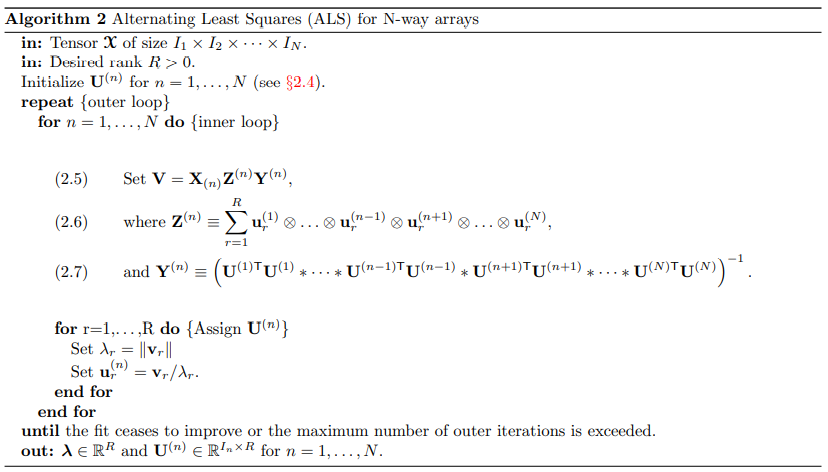
\includegraphics[width=420pt]{2.alg.png}  
    \label{fig:5}
\end{figure}


\subsubsection{Inicijalizacija}
\textbullet~ Pohlepni PARAFAC - inicijaliziramo matrice $\mathrm{U}^{(n)}$ kao matrice dobivene pohlepnim PARAFAC algoritmom\\
\textbullet~ Nasumična inicijalizacija - matrice $\mathrm{U}^{(n)}$ inicijaliziramo nasumičnim vrijednostima\\
\textbullet~ HOSVD inicijalizacija - za svaki mod $\mathrm{X}_{(n)}$ izračunamo SVD dekompoziciju, $\mathrm{X}_{(n)} = \mathrm{U}_{n}\Sigma_{n}\mathrm{V}_{n}^{T}$, i inicijaliziramo matrice $\mathrm{U}^{(n)} = \mathrm{U}_{n},~n = 1, \dots , N$

\subsection{Specijalna konsideracija za razbacane podatke}
Kao što smo već spomenuli, tenzor $\boldsymbol{\mathcal{X}}$ je veoma rijedak. Posljedično, njegova reprezentacija $\boldsymbol{X}_{n}$ je rijetka matrica (ima iste ne nul elemente, ali preoblikovane).
Matrica $\boldsymbol{Z}^{n}$ iz (2.6) se ne bi trebala formirati eksplicitno jer bi onda bila gusta matrice veličine $I_n \times J$ gdje je $J = \prod_{k = 1, k \neq n} ^{N} I_N$.
Umjesto toga, računanje
\begin{equation}
    \boldsymbol{X}_{(n)}\boldsymbol{Z}^{(n)}    
\end{equation}
potrebno za (2.5) mora biti izračunato posebno, iskorištavanjem svojstava Kroneckerove strukture produkta u $\boldsymbol{Z}^{(n)}$ da bi se očuvala rijetkost. Završni rezultat je veličine $I_n \times R$ stoga sse može pohraniti u gustu matricu.
Jedna od metoda prikazana je sljedećim algoritmom:

\begin{figure}[hbt!]
    \centering
    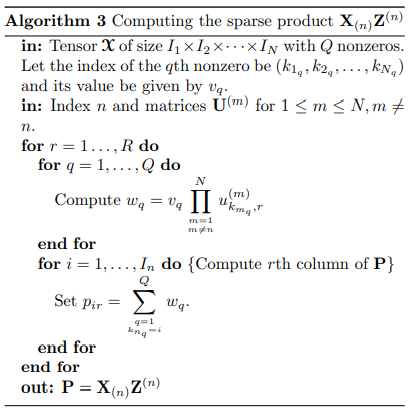
\includegraphics{3.alg.png}  
    \label{fig:5}
\end{figure}

\newpage
\section{TOPHITS i upiti}
Jednom kada smo izračunali TOPHITS model ranga $R$
\begin{equation}
   \boldsymbol{\mathcal{X} =  \lambda [\![ H, A, T ]\!]}
\end{equation}
možemo ga iskoristiti za razumijevanje podataka na razne načine.
Gledajući najveću vrijednost svake trojke $\{\boldsymbol{h_r}, \boldsymbol{a_r}, \boldsymbol{t_r}\}$ pruža grupiranje hubova, autoriteta, termova  web stranice, a $\lambda_r$ pruža relativnu težinu grupiranja.

Jedno pitanje koje smatramo osnovnim pitanjem web pretraživanja: pronaći sve stranice povezane s određenim termom ili skupom termova.
Promotrimo vektor upita $g$ duljine $K$ (gdje je $K$ broj termova) kao:


\begin{equation}
    q_{k} =  \left\{
	\begin{array}{ll}
		1  & \mbox{ako je term k u upitu} \\
		0 & \mbox{inače }
	\end{array}
\right.
\end{equation}

Primijetimo da nema razloga restringirati se na upite o termovima. Također se možemo baviti problem pronalaženja web stranica i/ili termova povezanih s određenom stranicom ili skupom stranica.

\subsection{Pronalaženje podudarne grupe}
Umjesto vraćanja liste rangiranih stranica, TOPHITS omogućuje opciju identificiranja grupiranja relevantnih za dani upit. Možemo kreirati vektor grupe $\boldsymbol{s}$ duljine $R$ koji sadrži vrijednosti svakog grupiranja, na temelju matrice $\boldsymbol{T}$ iz PARAFAC modela:
\begin{equation}\label{eq:311}
    \boldsymbol{s = \Lambda T^{T} q},  \boldsymbol{\Lambda} = diag(\boldsymbol{\lambda})
\end{equation}

Ulaz $s_r$ daje rezultat-vrijednost r-te grupe, a grupiranja s većim rezultatima smatraju se više relevantnima.

Alternativno, možemo konstruirati vektora upita na temelju web stranica, $\boldsymbol{\hat{q}} \in R^{l}$ te izračunati rezultate grupe kao:
\begin{equation}
    \boldsymbol{\hat{s} - \Lambda A^{T} \hat{q}},  \boldsymbol{\Lambda} = diag(\boldsymbol{\lambda})
\end{equation}

\subsection{Pronalaženje skupa autoriteta}
Također je moguće vratit tradicionalnu rangiranu listu vjerojatnosti. Možemo kombinirati sve informacije TOPHITS modela da bi vratili skup rangiranih autoriteta i/ili hubova.
Definirajmo $\boldsymbol{s}$ kao u \ref{eq:311}.
Tada su kombinirani autoriteti dani s:
\begin{equation}
    a^{*} = As = \sum_{r=1} ^{R} s_r a_r
\end{equation}

Sortiranje ulaza $\boldsymbol{a^{*}}$ vraća rangiranu listu autoriteta. Na isti način, kombinirani hubovi dani su:
\begin{equation}
    h^{*} = Hs = \sum_{r=1} ^{R} s_r h_r
\end{equation}

\newpage
\section{Implementacija}
Testirali smo našu tehniku na skupu podataka, generiranima koristeći web crawler koji uključuje i tekst poveznice.

\begin{lstlisting}
\end{lstlisting}


\end{document}

